\documentclass{beamer}
% This is the file main.tex
\usepackage[slantfont,boldfont]{xeCJK}
\usepackage{graphicx}
\setCJKmainfont{SimSun}
\usetheme{Berlin}
\title{机器学习框架}
\author{姜霄棠}
\date{\today}
\begin{document}
\begin{frame}
\titlepage
\end{frame}
\section*{Outline}
\begin{frame}
\tableofcontents
\end{frame}
\section{背景与目的}
\subsection{量化投资调研}
\begin{frame}{股票价格预测与决策}
\begin{itemize}
\item 对股票价格趋势进行时间序列分析
\item 预测走势,进行决策
\end{itemize}
\end{frame}
\subsection{机器学习算法的性能问题}
\begin{frame}{机器学习算法性能现状}
\begin{itemize}
\item 目前机器学习算法主要在服务器或学术研究中使用,其性能很少受到关注。
\item 大数据下的机器学习算法目前一般依赖scale out,但如果有易于扩展且性能完美的设计,机器的运算效果可以提升10倍,进而减少功耗。
\item 移动终端后面会越来越多地使用机器学习算法,目前普通使用的机器学习库不能满足性能功耗的要求。
\end{itemize}
\end{frame}

\begin{frame}{异构计算标准化}
\begin{itemize}
\item SIMD技术和GPU加速技术可使程序性能大幅上升。
\item 不同的机器上,由于硬件的不同,这些技术要么需要参数调优,要么完全不可用。
\end{itemize}
\includegraphics[height=0.5\textheight]{../pics/hibid.jpg}
\end{frame}
\subsection{自动编程实践}
\begin{frame}{自动编程框架}
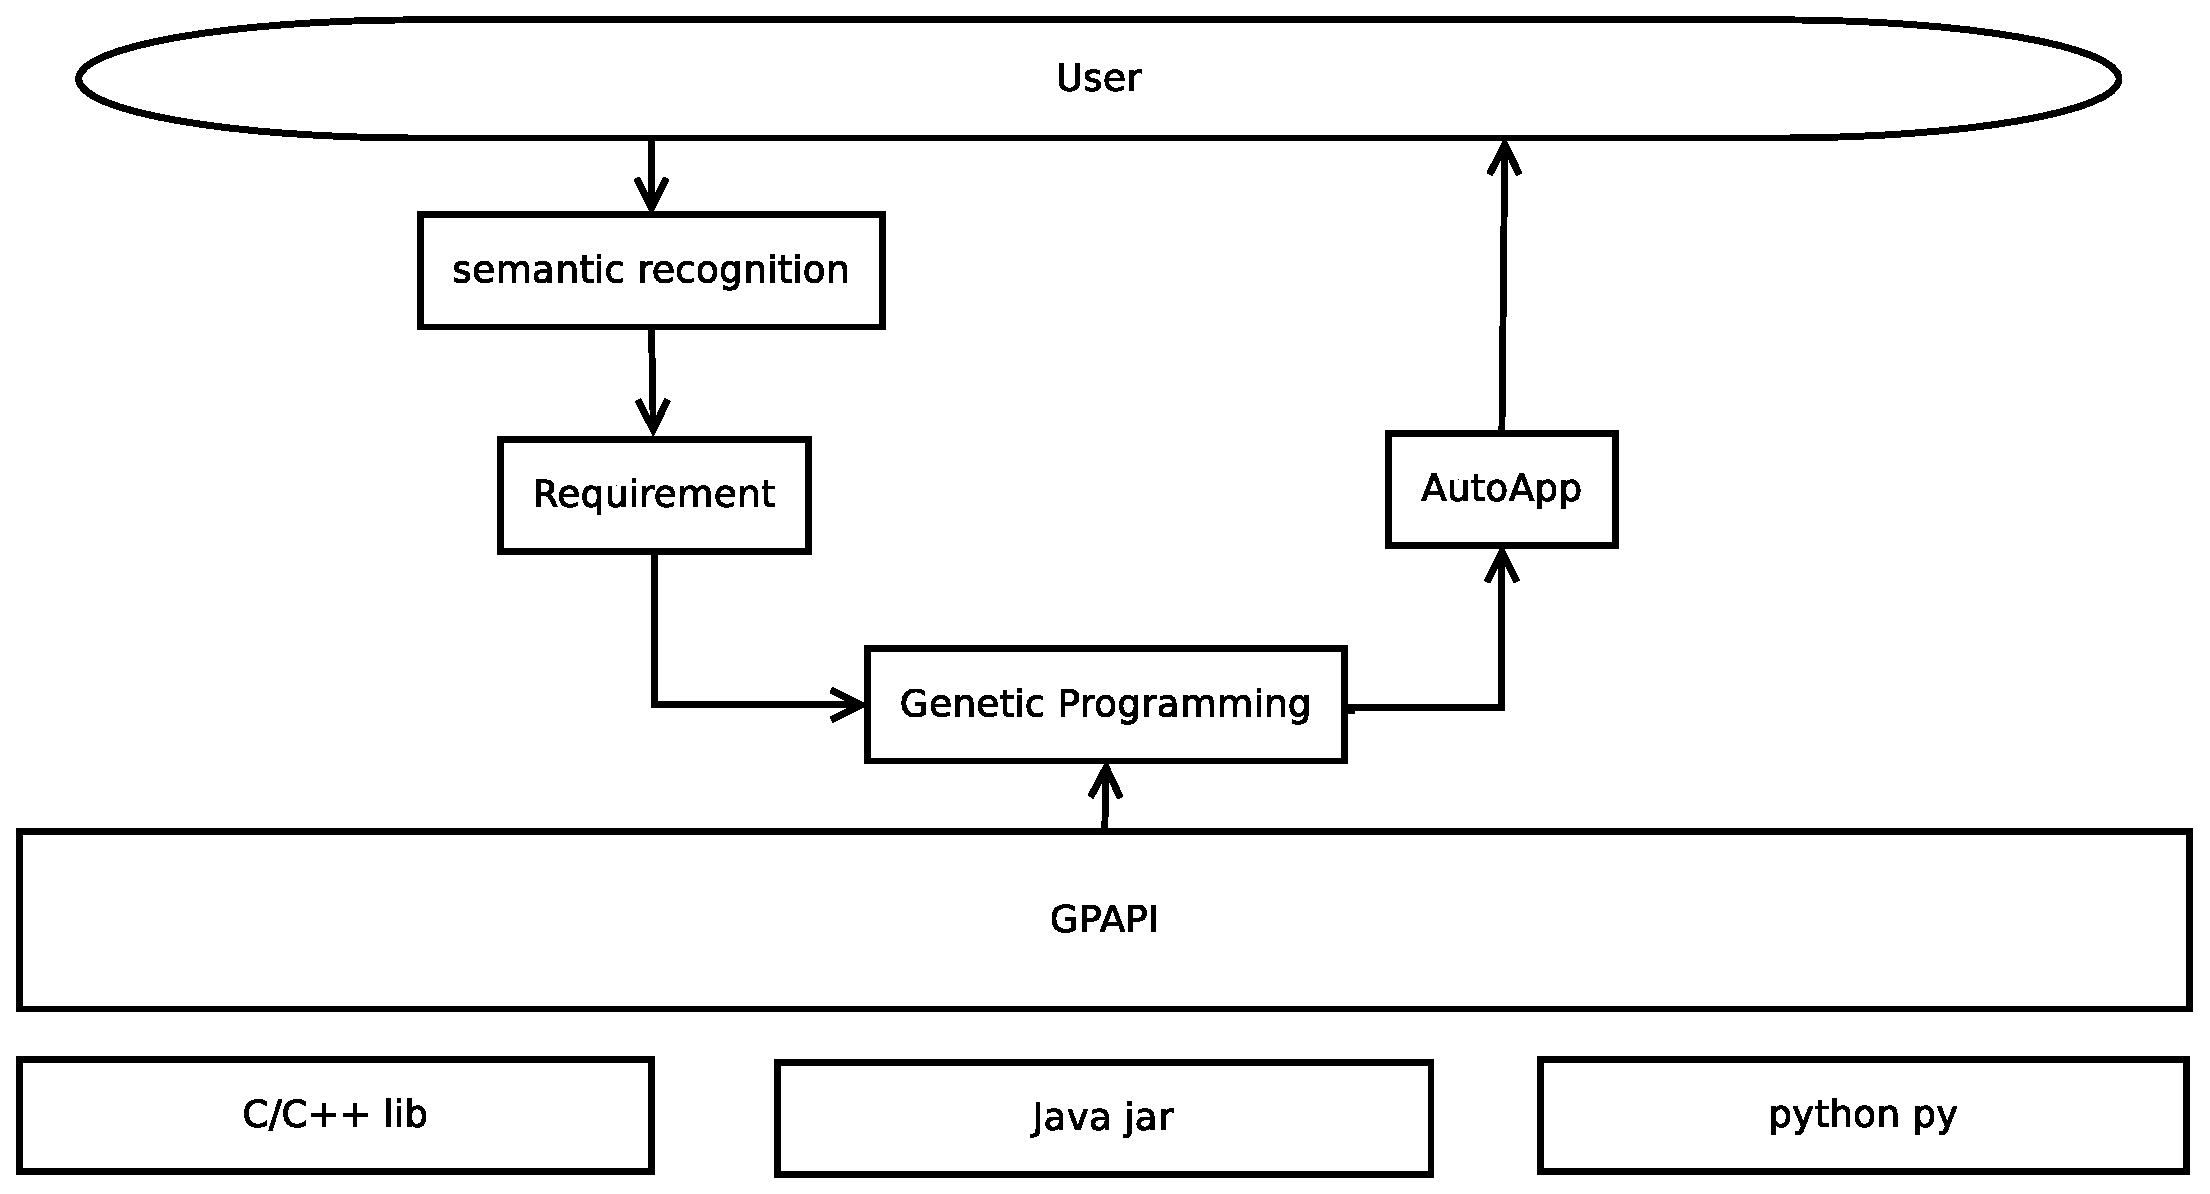
\includegraphics[height=0.8\textheight]{../pics/Frame.eps}
\end{frame}
\begin{frame}{目前GP框架的用法}
\begin{itemize}
\item 编写根函数代码,规定关联结构,最终函数可由根函数按一个xml表拼装而成。
\item 由GP框架学习xml结构,调整参数。
\item 学习出来的xml即Auto Program
\end{itemize}
\end{frame}
\section{机器学习相关算法}
\subsection{数据清洗}
\subsection{特征/成分提取}
\begin{frame}{时间序列}
\begin{itemize}
\item AR模型
\item 相空间重构
\end{itemize}
\end{frame}
\begin{frame}{图像相关}
暂不用关注
\begin{itemize}
\item 压缩感知
\item SIFT
\end{itemize}
\end{frame}
\begin{frame}{流形学习}
\begin{itemize}
\item 主成分分析(PCA)
\item 多维尺度分析
\end{itemize}
\end{frame}
\begin{frame}{数据转换}
\begin{itemize}
\item 小波变换
\item 标准化
\item 核函数映射
\end{itemize}
\end{frame}
\begin{frame}{预测:分类}
\begin{itemize}
\item 决策树
\item 随机森林(组合算法)
\item AdaBoost
\item KNN
\item SVM(组合算法)
\end{itemize}
\end{frame}
\begin{frame}{预测:回归}
\begin{itemize}
\item 最小二乘法
\item 逻辑回归
\item LU分解
\item CART(组合算法)
\end{itemize}
\end{frame}
\begin{frame}{定式优化算法}
\begin{itemize}
\item 梯度下降/随机梯度下降
\item 线性规划解法(单纯形法,内点法等)
\item 二次规划解法(SMO算法)
\end{itemize}
\end{frame}
\begin{frame}{深度学习}
深度学习是独立于以上算法的另一个分支。
\begin{itemize}
\item 自动编码器
\item 稀疏编码
\item 限制波尔兹曼机RBM与深信度网络
\item 卷积神经网络CNN
\end{itemize}
\end{frame}
\subsection{抽象层算法}
\begin{frame}{启发式优化算法}
这部分由GP框架层实现,不属于机器学习库的内容。
\begin{itemize}
\item 遗传算法
\item 粒子群算法
\item 模拟退火算法
\end{itemize}
\end{frame}
\section{开发任务与计划}
\subsection{基本时间序列预测功能实现}
\begin{frame}{需要实现的算法}
计划2月中旬完成。
\begin{itemize}
\item 决策树
\item 随机森林
\item SVM(已经完成)
\item AR模型回归(已经完成)
\item PCA
\item 小波变换(可选)
\end{itemize}
\end{frame}
\begin{frame}{股票预测模型}
计划2月底完成
\begin{itemize}
\item 数据提取
\item 价格预测
\item 执行器
\item 执行器评估
\end{itemize}
\end{frame}
\subsection{深度学习算法开发}
\begin{frame}{深度学习算法}
计划3月份完成
\begin{itemize}
\item 数据收集
\item 算法开发
\item 效果验证
\end{itemize}
\end{frame}
\subsection{GPU算法加速}
\begin{frame}{GPU算法加速}
计划4月份完成
\begin{itemize}
\item PCA
\item SVM
\item 深度学习
\item 线性回归
\end{itemize}
\end{frame} % to enforce entries in the table of contents
\end{document}
